\chapter{Level Set Methods}
\newcommand{\uxt}{$u(\mathbf{x}, t)$ }

A level set formulation is an implicit representation of a closed curve or curves. 
The curve is represented as a constant value of a function defined on a higher
dimensional domain. An example of this is level curves on a map. Provided 
a continuous function describing the hight of the mountain on the whole
domain, the contours joins points of equal elevation. In a cartographic
setting, there are numerous curves representing different elevations that 
are separated by a constant height. Thus contours are effectively describing
the steepness and height, and thus the shape, of the mountain. In a level set
context, we are not interested in the shape of the underlying higher dimensional
function, but we are very much interested in the contours, which we call 
\textit{iso-curves} or \textit{iso-contours}.

To continue with the cartographic image, 
The image of contours on a map is useful when understanding iso-curves in a
level set setting also. Since the level set formulation is a way of describing
closed curves, we need to know under which circumstances iso-contours forms 
closed curves. As we are used to from maps, elevation curves are always closed.

\todo{Fullfør. Kontinuitet?}

Now that we have an intuition about iso-curves, we can discuss the principle
of a level set method. The goal is to represent a closed curve or surface, 
$\Gamma(t)$, that moves under the influence of a velocity field $\vv{v}$.
The level set approach to this problem, as first presented in 1987 by 
S.Osher and J. Sethian \cite{MR965860}, is to define a continuous function
\uxt defined on a domain $\mathcal{D}$ containing $\Gamma|_{t=0}$.
The domain $\mathcal{D}$ is split in two parts by the curve $\Gamma$, the interior
$\Omega$ and the exterior $\mathcal{D} \setminus \Omega$. 
\begin{figure}
    \centering
    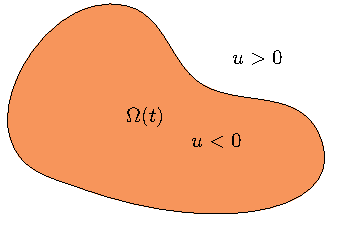
\includegraphics[width=.7\linewidth]{figures/tikz-figures/optimization-problem.pdf}
    \caption{Level set representation of a curve $\Gamma$}
    \label{fig:levelset-representation}
\end{figure}
The function \uxt must be constructed in a way that it satisfies the following properties
\begin{align}
    u(\mathbf{x}, t) < 0 \qquad &\text{for } \mathbf{x} \in  \mathfrak{I}(t) \label{eq:interior}\\
    u(\mathbf{x}, t) = 0 \qquad &\text{for } \mathbf{x} \in  \Gamma(t) \label{eq:zero-iso-curve}\\
    u(\mathbf{x}, t) > 0 \qquad &\text{for } \mathbf{x} \in  \mathfrak{O}(t) \label{eq:exterior}.
\end{align}
Now, the curve $\Gamma$ can be described in terms of \uxt by being its 
zero iso-contour. This means that if we can find the proper evolution of 
\uxt we can implicitly track the motion of the curve $\Gamma$.
What we now want is to find the right motion for \uxt to
track the level curve $\Gamma$ flowing in the velocity field $\vv{v}$. Because
we are only interested in the movement of the zero iso-curve of \uxt,
differentiate \eqref{eq:zero-iso-curve} with respect to time to find the movement
of $\Gamma$ when \uxt changes.
\begin{equation}
    (u(\mathbf{x}, t)_t + \nabla u(\mathbf{x}, t) \, \Gamma_t)_{\mathbf{x}\in \Gamma} = 0
    \label{eq:general-u-flow}
\end{equation}
When $\Gamma$ flows in the velocity field $\vv{v}$, its time derivative has to be 
defined as \todo{dette er ikke helt bra:}
\begin{equation}
    \Gamma_t = \vv{v}\cdot \vv{n}_{\Gamma} = v_n \vv{n}_{\Gamma}.
\end{equation}
In addition, we can see from \eqref{eq:interior}-\eqref{eq:exterior} that the gradient 
of $u$ at the curve $\Gamma$ is always pointing in the direction of the normal vector of 
$\Gamma$, $\vv{n}_{\Gamma}$. Thus we can write 
\begin{equation}
    \vv{n}_{\Gamma} = -\frac{\nabla u}{|\nabla u|}
\end{equation}

Inserting everything back into \eqref{eq:general-u-flow}, we get the equation
\begin{equation}
    u_t - v_n\, |\nabla u| = 0
    \label{eq:general-level-set}
\end{equation}

Now we have derived a PDE that will move surface or a curve under the influence
of a velocity field $\vv{v}$. However, there exists other methods to model
a moving surface and thus we ask the question: How does the level set 
formulation differ from other methods and in what situations could this be 
a preferred choice?




What to discuss around the method?
\begin{enumerate}
    \item increased complexity for solving PDE on entire domain. How to fix
    \item Topological flexibility. Situations that are now easily handled.
    \item Existence of viscosity solution (?????). In that case, I must read.
    \item Existence and uniqueness
\end{enumerate}

\newpage
\section{Level Set Formulation for Surfaces Approaching Unstructured and Irregular Point Sets}
Going back to our problem, we have a set of points sampled from a surface and we want to
reconstruct this surface as a smooth curve. Doing this using
a level set method means that given an initial curve $\Gamma_0$, we want to find the 
appropriate velocity field in \eqref{eq:general-level-set} such that the surface moves
closer and closer to the point set. In addition we want to ensure a smooth solution

We then try to find the optimal velocity field to enforce this behavior. In order
to do this, we formulate our problem as an optimization problem with respect to variations
of the surface $\Gamma$. The optimal change in $\Gamma$ is then the optimal speed for 
our curve. Extending that velocity to the entire domain gives us all the information we 
need to construct our level set formulation.
\todo{Discuss local property of the PDE}




